\scanpage{62}
\mspage{18}
One should make explicit a \uline{small} preliminary dévissage theorem, which will say that up to equivalence (defined up to unique isomorphisms)
$S_*\mathcal TD_{\mathrm{top}}^\pm$,
\inserted{with the functor $\Gamma$ into $(\mathrm{Gr.pond.}\unsure{\mathrm{rep}|\mathrm{top}})$ and $\unsure{\chi|f}$ into $[\pm1]$, and}
with the elementary operations $1^\circ$ to $7^\circ$ (or their simultaneous composite variants) is reconstructed from knowledge of the following groupoids and functors
\margin{\uline{with the exception of $4^\circ$ and $5^\circ$}}

\deleted{\diagram{\begin{tikzcd}[ampersand replacement=\&,row sep=large,column sep=large]
S_1\mathcal T_{g,\nu}^{\deleted{\unsure{0}}\pm}\arrow[r]\arrow[d]
\&{[\pm1]}\\
\unsure{\mathrm{Ens}(\nu)}
\end{tikzcd}}}
\deleted{\diagram{\begin{tikzcd}[ampersand replacement=\&]
\&\mathcal T_{g,\nu}^{\pm}\arrow[dl]\\
{}\&
\end{tikzcd}}}

$(*)$\quad
\diagram{\fbox{\begin{tikzcd}[ampersand replacement=\&,column sep=large]
S_1\mathcal T_{g,\nu}^\pm\arrow[r]
\&\mathcal T_{g,\nu}^\pm\arrow[r]
\&(\mathrm{Ens}(\nu)\times[\pm1])
\end{tikzcd}}}
\margin{(\unsure{we shall abbreviate as|we shall write|or simply} $S\mathcal T_{g\nu}^\pm$)}
\deleted{\unsure{$\varnothing$}}

$S_1\mathcal T_{g,\nu}^\pm$ denotes the subgroupoid of $S_*\mathcal T_{\mathrm{top}}^\pm$ consisting of the $(X,R)$ such that $X$ is connected of genus $g$, $\operatorname{card}\pi_0\partial X=\nu$, and $\operatorname{card}R\cap C_a=1$ (for every $a\in\pi_0\partial X$ --- that is, the \inserted{doubly weighted} graph of the
$\deleted{\unsure{\mathcal T_{g,\nu}}}(X,\underset{\Vert\,\partial X}{\widetilde\Sigma},R)$ is isomorphic to
\figure{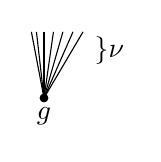
\begin{tikzpicture}[scale=.8]
\fill (0,0) circle(2pt);
\node[below] at (0,0) {$g$};
\foreach \x in {-.2,-.12,0,.15,.3,.46,.62}{\draw (0,0)--(\x,1.05);}
\node[right] at (.65,.75) {$\}\nu$};
\end{tikzpicture}}
all these edges (free) have weight 1

and $\mathcal T_{g,\nu}^\pm$ is defined in a corresponding way, via the $(X,\varnothing,\varnothing)$ where $X$ of type $g,\nu$.

\margin{This is not quite enough, to \unsure{reconstruct|have all} the operations In particular the operations
\textcircled{$4^\circ$} (which \unsure{requires} some \deleted{\unsure{links}} \inserted{\unsure{``or''|the introduction}} \unsure{structures} \unsure{$\mathcal T_{g,\infty}$|$\mathcal T_{g,\nu}$}) and \textcircled{$5^\circ$}}
\mspage{61}
